\documentclass[11pt]{article}

\usepackage[margin=1in]{geometry}
\usepackage{setspace}
\usepackage{amsmath}
\usepackage{amssymb}
\usepackage{booktabs}
\usepackage{array}
\usepackage{longtable}
\usepackage{graphicx}
\usepackage{float}
\usepackage{caption}
\usepackage{url}
\usepackage{hyperref}
\usepackage{xcolor}
\usepackage{enumitem}


\usepackage[numbers,sort&compress]{natbib}

\hypersetup{colorlinks=true, linkcolor=black, citecolor=black, urlcolor=blue}


\title{
\textbf{Bayesian Logistic Regression of Diabetes Risk in NHANES (2021--2023):\\
Evaluating Informative Priors Transferred From NHANES 2013--2014}
}

\author{
Namita Mishra, MD, MS, MPH$^{1,*}$ \and
Ashraf Cohen, PhD, MS$^{2}$
}

\date{}  % Remove the automatic date

\begin{document}

\maketitle

\noindent
$^{1}$ University of West Florida, Usha Kundu College of Health,
Pensacola, Florida, USA\\
$^{2}$ University of West Florida, Pensacola, Florida, USA\\
$^{*}$ Corresponding author


\begin{abstract}

\textbf{Background:} Bayesian logistic regression allows prior information
from earlier studies to inform estimation in new data. This study evaluated
whether posterior information from a prior NHANES cycle (2013--2014) improves
Bayesian estimation of diabetes risk in a subsequent NHANES cycle (August
2021--August 2023).

\textbf{Methods:} Adults aged $\geq20$ years from NHANES August
2021--August 2023 ($N=7{,}809$) were analyzed after excluding missing data in diabetes outcomes yielding a total of 7,536 adults. Missing BMI (23.5\%) was addressed using multiple imputation by chained equations
(MICE). Standardized age and BMI, sex, and race/ethnicity were modeled
using survey-weighted frequentist logistic regression and two Bayesian
models: weakly informative Normal$(0,2.5)$ priors and informative priors
derived from the NHANES 2013--2014 posterior for harmonized predictors
(intercept, age, BMI, and sex). Race/ethnicity priors were not transferred
because category definitions differed between cycles. Bayesian models used
\texttt{brms}/Stan with normalized examination weights, four chains,
2,000 iterations, 1,000 warmup iterations, and
\texttt{adapt\_delta}=0.95.

\textbf{Results:} Age (survey-weighted OR~$=2.84$, 95\% CI: 2.45--3.31;
weak-prior Bayesian OR~$=2.85$, 95\% CrI: 2.60--3.12; informative-prior
Bayesian OR~$=2.88$, 95\% CrI: 2.63--3.14) and BMI (survey-weighted
OR~$=1.84$; weak-prior OR~$=1.85$; informative-prior OR~$=1.86$) were the
strongest predictors of diabetes across all three models. Female sex was
associated with lower odds (weak-prior OR~$=0.72$; informative-prior
OR~$=0.69$). Black, Hispanic, Asian, and Other race/ethnicity groups all had
higher odds than White across models. Informative and weak
priors produced nearly identical posterior estimates for age, BMI, and race
(percent differences generally $<1.5\%$), with a somewhat larger shift for
sex (OR 0.72 to 0.69, a 3.3\% change), indicating limited prior-data
conflict. Leave-one-out cross-validation showed no meaningful predictive
advantage for the informative-prior model over the weak-prior model
(elpd difference~$=-0.2$, SE~$=0.7$). Bayesian model-based posterior diabetes
prevalence was 14.9\% for both models, compared with a survey-weighted
prevalence of approximately 12.1\% and an unweighted sample prevalence of
14.2\%.

\textbf{Conclusions:} Cycle-1-informed priors produced posterior estimates
nearly identical to weakly informative priors and did not improve predictive
performance in NHANES Cycle 2, indicating that the large Cycle 2 sample
dominated the likelihood and that no material prior-data conflict was
present for the harmonized predictors (age, BMI, sex). Age and BMI remained
the strongest and most consistent predictors of diabetes across both NHANES
cycles and both frequentist and Bayesian frameworks. As in Cycle 1, Bayesian
model-based prevalence exceeded the design-based survey-weighted estimate,
reinforcing that normalized examination weights alone do not reproduce
design-based population inference.

\end{abstract}

\noindent\textbf{Keywords:} Bayesian logistic regression; diabetes;
NHANES; informative priors; prior transfer; survey-weighted regression;
posterior predictive checking; complex survey data.

\section{Introduction}


Diabetes mellitus remains a major public health challenge in the
United States. Its burden is strongly associated with age, adiposity,
sex, and race/ethnicity, while socioeconomic and structural factors
also contribute to observed disparities \citep{Gwira2024}.

Bayesian logistic regression framework allows incorporating prior information into epidemiologic analyses. In Bayesian logistic regression
parameters are represented by probability distributions. Posterior distributions combine likelihood information with prior distributions and provide
direct measures of uncertainty through credible intervals and posterior pre-
dictions [5, 9, 18]. 
Bayesian methods have also been applied to diabetes
2
risk prediction using National Health and Nutrition Examination Survey
(NHANES) data [16]


Bayesian analysis of successive survey cycles raises a specific
methodological question that is distinct from single-cycle analysis: whether
posterior information from an earlier cycle can be transferred as prior
information for a later cycle, and whether doing so meaningfully changes or
improves estimation. Weakly informative priors are commonly used by default
in Bayesian regression to provide light regularization without imposing
strong assumptions about the direction or magnitude of an association
\citep{Gelman2008}. An alternative approach is to construct priors directly
from a finalized posterior obtained in an earlier, related dataset, which in
principle allows cumulative evidence to inform new analyses
\citep{Kruschke2017,VandeSchoot2021}.

This prior-transfer approach requires that the outcome definition,
predictor definitions, reference categories, and standardization procedures
be harmonized across the two datasets before posterior-derived priors are
transferred directly; when full harmonization is not possible for a given
predictor, that predictor should retain a weakly informative rather than an
informative prior \citep{Baldwin2017,Hoeting1999}. Comparing models fit with
weakly informative priors and with informative priors derived from a prior
cycle also provides a natural sensitivity analysis: close agreement between
the two supports robustness of the underlying association, whereas
meaningful divergence may indicate either genuine change in the population
between cycles or an important difference in how variables were defined or
measured \citep{Ospel2024,VandeSchoot2021}.
The implementation of Bayesian methods allows sensitivity analyzes to assess the robustness of study findings to misclassification and missing data \cite{Luta2013Bayesian}. Prior sensitivity analysis is therefore important when Bayesian methods are used for epidemiologic inference. A model that produces similar estimates under weakly informative and informative priors provides evidence that conclusions are relatively robust to prior specification. Conversely, substantial differences may indicate that posterior inference is meaningfully influenced by prior information. 

The present study therefore uses a repeated cross-sectional (RCS) Bayesian
logistic regression framework to evaluate whether posterior information
from an earlier NHANES cycle can be transferred as informative prior
information to a subsequent independent cross-sectional sample
\cite{Eisinga2002,Steyn2025}. Comparison with weakly informative priors
provides a direct assessment of the sensitivity of posterior estimates to
prior specification.

This study is based on a completed Bayesian and survey-weighted logistic
regression analysis of doctor-diagnosed diabetes using NHANES 2013--2014 (Cycle-1, ~ref\ ),
in which age and BMI were the strongest predictors of diabetes, female sex
was associated with lower odds, and several racial/ethnic groups showed
higher odds relative to the reference category. Specifically, the current study compared a Bayesian model using weakly informative priors with a Bayesian model using informative priors derived from posterior estimates obtained from NHANES 2013--2014. 

 
\subsection{Objectives}

The primary objectives of this study were to:

\begin{enumerate}[label=(\roman*)]
    \item estimate the associations of age, BMI, sex, and race/ethnicity with
    doctor-diagnosed diabetes among adults in NHANES August 2021--August
    2023; and

    \item evaluate whether informative priors derived from the NHANES
    2013--2014 Bayesian posterior materially changed posterior estimates
    compared with weakly informative priors.
\end{enumerate}

The secondary objectives were to:

\begin{enumerate}[label=(\roman*)]
    \item compare Bayesian estimates obtained using weakly informative priors
    with estimates from survey-weighted frequentist logistic regression;

    \item compare the predictive performance of the weak-prior and
    Cycle-1-informed-prior Bayesian models using leave-one-out cross-validation;

    \item assess whether the direction and magnitude of associations observed
    in NHANES 2013--2014 were broadly consistent with those observed in
    NHANES August 2021--August 2023; and

    \item compare Bayesian model-based posterior diabetes prevalence with the
    design-based survey-weighted prevalence estimate.
\end{enumerate}
 





\section{Methods} 


\subsection{Study Design}


The study used a repeated cross-sectional (RCS) Bayesian logistic regression
framework based on two independent NHANES cycles \cite{Stival2026}. Bayesian analysis of complex survey data requires careful consideration of
informative sampling and survey weights because the sample distribution may
differ from the target population distribution \cite{Savitsky2024Informative} . Bayesian data-combination approaches have also
demonstrated that posterior information from an earlier dataset can serve as
prior information for subsequent analyses of RCS data
\cite{PelzerEisinga2002}. Building on these approaches, posterior information from
NHANES 2013--2014 \cite{CDC20132014NHANES} was transferred to construct informative priors for
selected harmonized predictors in NHANES August 2021--August  \citep{NCHS2023}. The
informative-prior and weakly informative-prior models were compared to
evaluate prior sensitivity and predictive performance. Because the two
NHANES cycles represent independent cross-sectional samples rather than
repeated measurements of the same individuals, the study was not
longitudinal \cite{Lebo2015}

 \subsection{Data Source and Study Population}
This study used the NHANES August 2021--August 2023 data release, the first
NHANES cycle conducted after the suspension of NHANES field operations in
March 2020 and reflecting an updated sample design \citep{NCHS2023}.
Demographic (DEMO\_L), body-measurement (BMX\_L), and diabetes (DIQ\_L)
component files were merged on the participant identifier SEQN using the
\texttt{haven} package in R. 

The analysis was restricted to adults aged 20
years and older, yielding 7,809 participants. Of these, 273 participants
(3.5\%) had a missing diabetes diagnosis and were excluded, leaving a final
analytic cohort of 7,536 adults with an observed diabetes outcome.  








\subsection{Ethical Considerations, Informed Consent, and Participant Incentives}

NHANES protocols were reviewed and approved by the National Center for
Health Statistics (NCHS) Ethics Review Board (ERB) \cite{CDC2026NHANESERB}.
Participation was voluntary, with informed consent obtained for household
interviews and Mobile Examination Center (MEC) examinations. To reduce barriers to participation, NHANES provided financial
incentives; during August 2021--August 2023, participants received \$25
after completing the household interview, with additional incentives for
MEC examination completion
\cite{Terry2024NHANES}. The present study used de-identified, publicly
available NHANES data and involved no direct participant contact;
therefore, additional institutional review board (IRB) review was not
required. 



\subsection{Variables}
The outcome, doctor-diagnosed diabetes (\texttt{diabetes\_dx}), was coded
0 (no) or 1 (yes) from the NHANES diabetes questionnaire. Age
(\texttt{age\_c}) and BMI (\texttt{bmi\_c}) were standardized (z-scored) so
that odds ratios reflect a one-standard-deviation increase, consistent with
the Cycle 1 analysis. Sex was coded as Male (reference) or Female.
Race/ethnicity was derived from RIDRETH3 and coded into five categories:
White (reference), Black, Hispanic, Asian, and Other. This categorization
differs from the five-category race/ethnicity variable used in the
NHANES 2013--2014 analysis (Non-Hispanic White, Mexican American, Other
Hispanic, Non-Hispanic Black, Other/Multi-racial); in particular, Cycle 2
distinguishes an Asian category not separately identified in Cycle 1, and
combines Hispanic-origin participants into a single category rather than
distinguishing Mexican American from Other Hispanic. Because of this
non-equivalence, race/ethnicity coefficients were treated as unharmonized
across cycles (see Section~2.5). 
Table~\ref{tab:sample} summarizes the descriptive characteristics of the
analytic cohort.

\begin{table}[H]
\centering
\caption{Descriptive Characteristics of the NHANES Cycle 2 Analytic Cohort
($N=7{,}536$)}
\label{tab:sample}
\begin{tabular}{lr}
\toprule
\textbf{Characteristic} & \textbf{Value} \\
\midrule
Age, years (mean, SD) & 53.3 (17.6) \\
BMI, kg/m$^2$ (mean, SD) & 29.7 (7.3) \\
Female, n (\%) & 4,171 (55.3\%) \\
Male, n (\%) & 3,365 (44.7\%) \\
\midrule
\multicolumn{2}{l}{\textbf{Race/ethnicity, n (\%)}} \\
White & 4,419 (58.6\%) \\
Hispanic & 1,275 (16.9\%) \\
Black & 959 (12.7\%) \\
Other & 497 (6.6\%) \\
Asian & 386 (5.1\%) \\
\midrule
Doctor-diagnosed diabetes, n (\%) & 1,070 (14.2\%) \\
\bottomrule
\end{tabular}
\end{table}

\subsection{Missing Data}
Among the 7,809 adults with an observed or missing diabetes outcome, BMI was
missing for 1,839 participants (23.5\%), a substantially higher missingness
rate than in the NHANES 2013--2014 analysis (4.3\%), consistent with the
updated data-collection procedures used in this post-pandemic NHANES cycle
\citep{NCHS2023}. Missing BMI was addressed using multiple imputation by
chained equations (MICE) with predictive mean matching, following the same
general approach used in the Cycle 1 analysis. The diabetes outcome itself
was not imputed. Age, sex, race, and NHANES survey design variables
(examination weight, primary sampling unit, stratum) had no missing values.
As in the Cycle 1 analysis, the Bayesian models were fit to the first
completed imputed dataset rather than pooled across multiple imputations;
this limitation is discussed further in Section~5.

\subsection{Survey-Weighted Logistic Regression}
Survey-weighted logistic regression was fitted using \texttt{svyglm()} with
a quasibinomial family, incorporating the NHANES examination weight, primary
sampling unit, and stratum to account for the complex survey design.
Continuous predictors were interpreted per one-standard-deviation increase;
male sex and White race/ethnicity were reference categories.

\subsection{Bayesian Logistic Regression and Prior Specification}
For participant $i$,
\begin{equation}
Y_i \sim \text{Bernoulli}(p_i), \qquad
\text{logit}(p_i) = \beta_0 + \beta_1 age_{c,i} + \beta_2 bmi_{c,i}
+ \beta_3 sex_i + \boldsymbol{\beta}_4 race_i,
\end{equation}
fitted using \texttt{brms}/Stan with normalized examination weights as
observation-level model weights, four MCMC chains, 2,000 iterations per
chain (1,000 warmup, 4,000 post-warmup draws), and
\texttt{adapt\_delta}~$=0.95$.

Two prior specifications were compared:

\textbf{Weak-prior model.} Regression coefficients were assigned weakly
informative Normal$(0,2.5)$ priors, matching the baseline specification used
in the Cycle 1 analysis.
\textbf{Informative-prior model.} Bayesian sensitivity analyses can use
informative priors to assess the influence of prior assumptions on
regression estimates \cite{Luta2013Bayesian}. In the present study,
informative priors were constructed directly from the finalized
NHANES 2013--2014 Bayesian posterior for coefficients with harmonized
definitions across cycles (intercept, age, BMI, and sex). Prior standard
deviations were set to 0.25 to provide informative but not overly
restrictive prior information relative to the Cycle 2 sample size:
\begin{align}
\beta_0 &\sim \text{Normal}(-2.6633,\ 0.25^2) \\
\beta_{age} &\sim \text{Normal}(1.0969,\ 0.25^2) \\
\beta_{bmi} &\sim \text{Normal}(0.6282,\ 0.25^2) \\
\beta_{sexFemale} &\sim \text{Normal}(-0.6625,\ 0.25^2)
\end{align}
Because race/ethnicity categories were not equivalent across cycles
(Section~2.2), race coefficients in the informative-prior model retained the
same weakly informative Normal$(0,2.5)$ prior used in the weak-prior model,
consistent with the harmonization requirement that posterior-derived priors
should not be transferred for predictors without matching definitions and
reference categories across cycles.

\subsection{Model Comparison and Evaluation}
Odds ratios were obtained by exponentiating posterior coefficients, with
95\% credible intervals from posterior quantiles. Convergence was assessed
using $\hat{R}$ and bulk/tail effective sample size (ESS). The weak-prior and
informative-prior models were compared directly using leave-one-out
cross-validation (LOO-CV) with the \texttt{loo} package. Calibration was
assessed by comparing mean predicted probability with observed diabetes
prevalence across deciles of predicted risk. Model-based posterior diabetes
prevalence was compared with the design-based survey-weighted prevalence
estimate, as in the Cycle 1 analysis. All analyses were conducted in R.

\section{Results}

\subsection{Study Population}
The NHANES Cycle 2 analytic cohort included 7,536 adults aged 20 years and
older with an observed diabetes diagnosis (Table~\ref{tab:sample}). Mean age
was 53.3 years (SD 17.6) and mean BMI was 29.7 kg/m$^2$ (SD 7.3). The cohort
was 55.3\% female. White participants comprised 58.6\% of the cohort,
followed by Hispanic (16.9\%), Black (12.7\%), Other (6.6\%), and Asian
(5.1\%) participants. Doctor-diagnosed diabetes was present in 14.2\% of the
unweighted analytic sample.

\subsection{Survey-Weighted Logistic Regression}
Age (OR~$=2.84$, 95\% CI: 2.45--3.31) and BMI (OR~$=1.84$, 95\% CI:
1.70--2.01) were the strongest predictors of diabetes diagnosis. Female
participants had lower odds than males (OR~$=0.71$, 95\% CI: 0.59--0.87).
Relative to White participants, odds were higher for Black (OR~$=2.31$,
95\% CI: 1.60--3.34), Hispanic (OR~$=1.83$, 95\% CI: 1.24--2.69), Asian
(OR~$=2.14$, 95\% CI: 1.31--3.49), and Other (OR~$=2.01$, 95\% CI:
1.37--2.94) participants.

\subsection{Weak-Prior and Informative-Prior Bayesian Models}
Both Bayesian models converged satisfactorily ($\hat{R}=1.00$ for all
parameters; bulk/tail ESS $>2{,}600$ throughout). Posterior estimates from
both models closely matched the survey-weighted results
(Table~\ref{tab:or_comparison}). In the weak-prior model, age OR~$=2.85$
(95\% CrI: 2.60--3.12) and BMI OR~$=1.85$ (95\% CrI: 1.71--1.98); in the
informative-prior model, age OR~$=2.88$ (95\% CrI: 2.63--3.14) and BMI
OR~$=1.86$ (95\% CrI: 1.73--2.00). Female sex was associated with lower
odds in both models (weak-prior OR~$=0.72$, 95\% CrI: 0.61--0.83;
informative-prior OR~$=0.69$, 95\% CrI: 0.60--0.80). Black, Hispanic, Asian,
and Other participants all had higher odds than White participants in both
models, with estimates nearly identical between the weak-prior and
informative-prior specifications (Table~\ref{tab:or_comparison}).
\begin{table}[H]
\centering
\small
\setlength{\tabcolsep}{4pt}

\caption{Odds Ratios for Doctor-Diagnosed Diabetes by Model}
\label{tab:or_comparison}

\begin{tabular}{lccc}
\toprule
\textbf{Predictor} &
\textbf{SW OR (95\% CI)} &
\textbf{Weak Bayes OR (95\% CrI)} &
\textbf{Informative Bayes OR (95\% CrI)} \\
\midrule

Age, 1 SD
& 2.84 (2.45--3.31)
& 2.85 (2.60--3.12)
& 2.88 (2.63--3.14) \\

BMI, 1 SD
& 1.84 (1.70--2.01)
& 1.85 (1.71--1.98)
& 1.86 (1.73--2.00) \\

Female vs Male
& 0.71 (0.59--0.87)
& 0.72 (0.61--0.83)
& 0.69 (0.60--0.80) \\

Black vs White
& 2.31 (1.60--3.34)
& 2.30 (1.83--2.85)
& 2.31 (1.85--2.90) \\

Hispanic vs White
& 1.83 (1.24--2.69)
& 1.82 (1.47--2.23)
& 1.83 (1.47--2.27) \\

Asian vs White
& 2.14 (1.31--3.49)
& 2.12 (1.48--2.95)
& 2.15 (1.50--3.07) \\

Other vs White
& 2.01 (1.37--2.94)
& 1.99 (1.50--2.63)
& 2.01 (1.50--2.69) \\

\bottomrule
\end{tabular}

\begin{flushleft}
\footnotesize
\textit{Note:} SW = survey-weighted; Bayes = Bayesian;
CI = confidence interval; CrI = credible interval.
Reference categories: Male (sex) and White (race/ethnicity).
\end{flushleft}

\end{table}
\subsection{Comparison of Weak-Prior and Informative-Prior Models}
Table~\ref{tab:sensitivity} summarizes the percent difference in posterior
odds ratios between the weak-prior and informative-prior models. Agreement
was close for age (0.95\% difference), BMI (0.76\%), and all four
race/ethnicity terms (0.62\%--1.41\%, consistent with these terms retaining
the same weakly informative prior in both models and differing only due to
posterior sampling variation). The largest shift was observed for sex
(3.31\% difference in OR, from 0.72 to 0.69), reflecting the informative
prior's pull toward the larger protective effect of female sex estimated in
NHANES 2013--2014 ($\beta_{sexFemale}=-0.6625$). Bayesian model-based
posterior diabetes prevalence was nearly identical between the two models
(informative-prior: 14.87\%, 95\% interval 14.05\%--15.72\%; weak-prior:
14.91\%, 95\% interval 14.10\%--15.79\%).



\begin{table}[H]
\centering
\caption{Prior Sensitivity: Comparison of Weak-Prior and Informative-Prior
Posterior Odds Ratios}
\label{tab:sensitivity}
\begin{tabular}{lrrr}
\toprule
\textbf{Term} & \textbf{OR (Weak Prior)} & \textbf{OR (Informative Prior)} &
\textbf{Percent OR Change} \\
\midrule
Intercept & 0.10 & 0.10 & $-0.31\%$ \\
Age, per 1 SD & 2.85 & 2.88 & $0.96\%$ \\
BMI, per 1 SD & 1.85 & 1.86 & $0.76\%$ \\
Female vs Male & 0.72 & 0.69 & $-3.20\%$ \\
Black vs White & 2.30 & 2.31 & $0.63\%$ \\
Hispanic vs White & 1.82 & 1.83 & $0.69\%$ \\
Asian vs White & 2.12 & 2.15 & $1.41\%$ \\
Other vs White & 1.99 & 2.01 & $0.81\%$ \\
\bottomrule
\end{tabular}
\end{table}


\begin{figure}
    \centering
    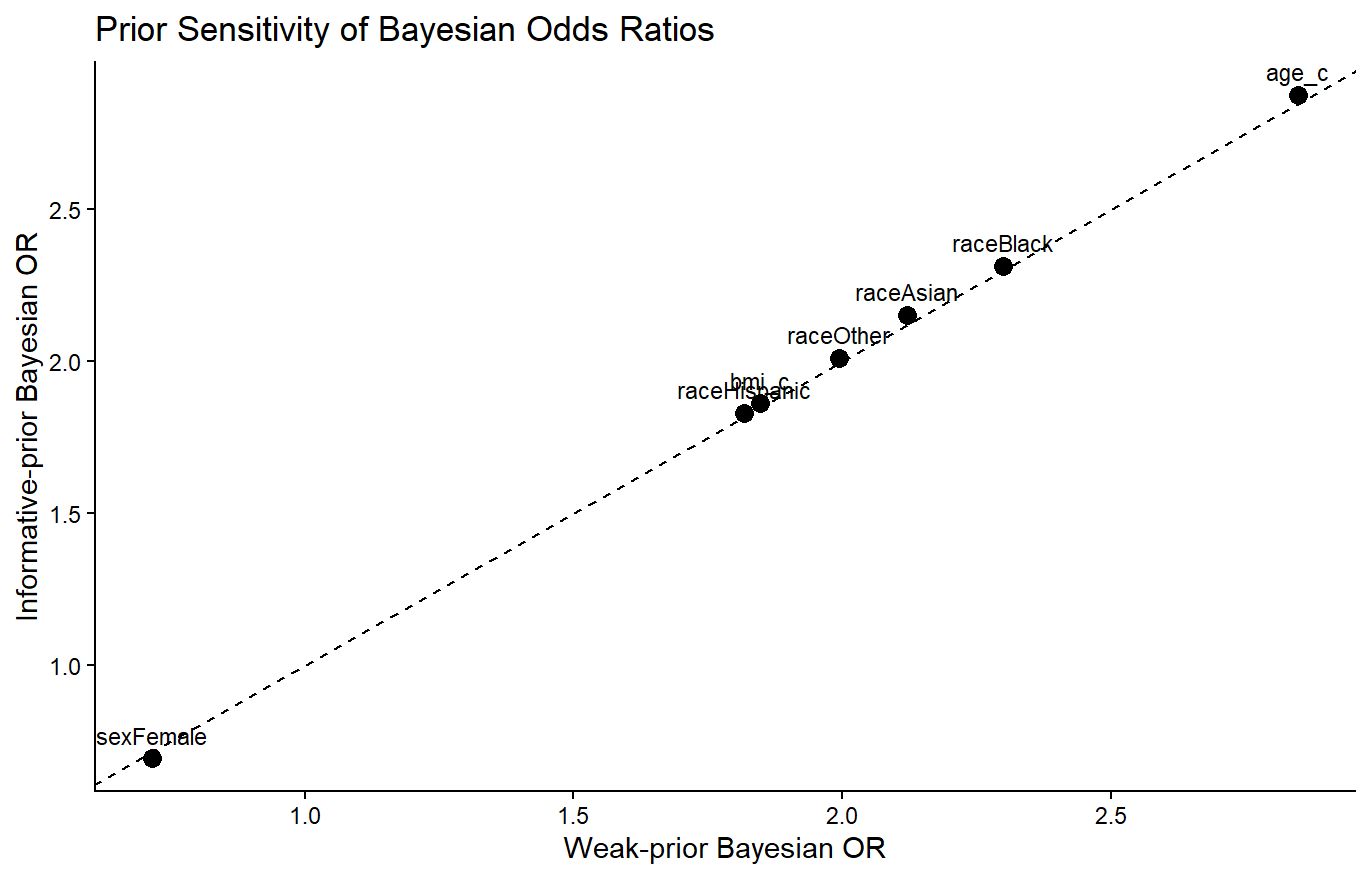
\includegraphics[width=0.5\linewidth]{Rplot_prior sensitivity_wealvsinformative OR comparision.png}
    \caption{Prior Sensitivity: Comparison of Weak-Prior and Informative-Prior Posterior Odds Ratios}
    \label{fig:placeholder}
\end{figure}
\begin{table}[H]
\centering
\caption{Diabetes Prevalence by NHANES Cycle and Prior Specification}
\label{tab:prior_prevalence}
\small
\setlength{\tabcolsep}{4pt}
\begin{tabular}{@{}l@{\hspace{8pt}}r@{\hspace{8pt}}r@{\hspace{8pt}}r@{\hspace{8pt}}r@{\hspace{8pt}}r@{}}
\toprule
\textbf{Cycle} &
\textbf{N} &
\textbf{SW (\%)} &
\textbf{Weak (\%)} &
\textbf{Info (\%)} &
\textbf{$\Delta$ (pp)} \\
\midrule
2013--2014 & 5,769 & 8.90 & 10.95 & -- & -- \\
2021--2023 & 7,536 & 12.10 & 14.91 & 14.87 & 0.04 \\
\bottomrule
\end{tabular}

\begin{flushleft}
\footnotesize
\textit{Note:} SW = survey-weighted; Weak = weakly informative
Bayesian prior; Info = informative Bayesian prior; $\Delta$ =
difference between weak-prior and informative-prior posterior
prevalence; pp = percentage points. Values are percentages.
The informative prior for 2021--2023 was derived from the
2013--2014 posterior.
\end{flushleft}
\end{table}
\subsection{Predictive Comparison of Weak-Prior and Informative-Prior Models}
Leave-one-out cross-validation showed no meaningful difference in predictive
performance between the two Bayesian specifications (elpd
difference~$=-0.2$, SE~$=0.7$, favoring the weak-prior model by a negligible
margin). Pareto-$k$ diagnostics flagged a substantial number of observations
with $k>0.7$ in both models, indicating that PSIS-LOO estimates should be
interpreted cautiously in the presence of the weighted likelihood used here
(see Limitations).

\subsection{Calibration}
Calibration across deciles of predicted risk showed close agreement between
mean predicted probability and observed diabetes prevalence throughout the
range of predicted risk, including at the highest-risk decile (mean
predicted probability 0.448 versus observed prevalence 0.377 in the top
decile, $n=753$).
\begin{figure}[H]
    \centering
    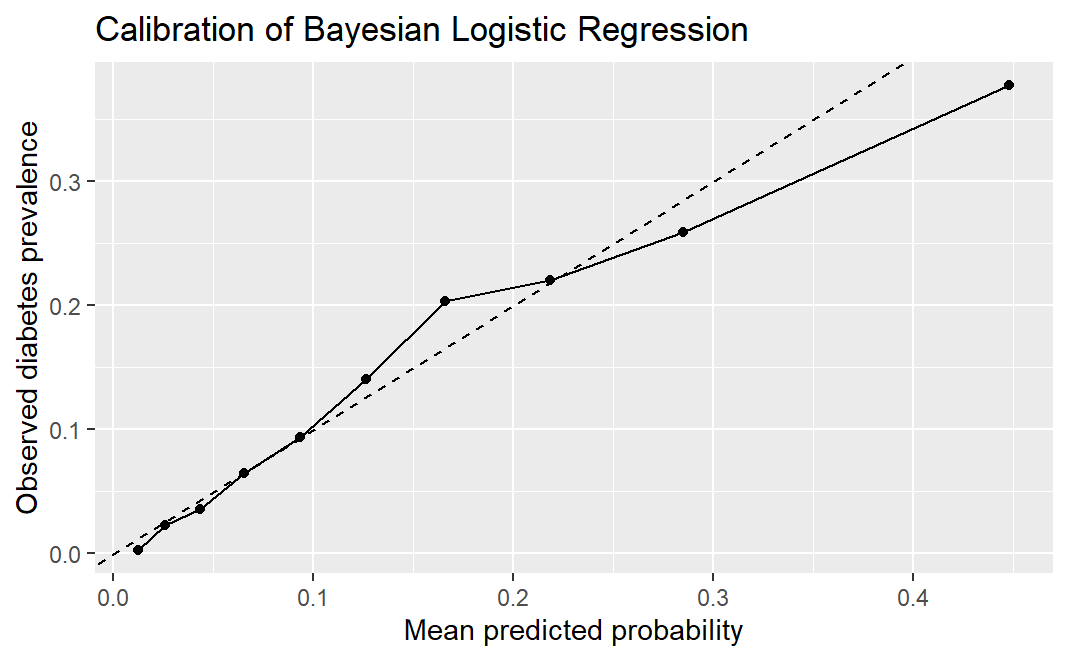
\includegraphics[width=0.5\linewidth]{claibration_cyc2.png}
    \caption{Calibration across deciles of predicted risk }
    \label{fig:placeholder}
\end{figure}


\subsection{Model-Based versus Design-Based Prevalence}
The Bayesian model-based posterior prevalence of diabetes (14.9\% for both
weak-prior and informative-prior models) exceeded the survey-weighted,
design-based prevalence estimate (approximately 12.1\%) and was closer to
the unweighted sample prevalence (14.2\%). This pattern parallels the
NHANES 2013--2014 analysis, in which Bayesian model-based prevalence
(10.95\%) similarly exceeded the design-based estimate (8.9\%), and is
consistent with the Bayesian models' use of normalized examination weights
rather than full incorporation of NHANES stratification and clustering into
the likelihood.

\section{Discussion}

This study evaluated whether Bayesian posterior information from NHANES
2013--2014 improved estimation of diabetes risk when transferred as
informative priors to NHANES August 2021--August 2023. Age and BMI remained
the strongest predictors of doctor-diagnosed diabetes in Cycle 2, consistent
in direction and approximate magnitude with the earlier cycle (Cycle 1 age
OR~$=2.99$ Bayesian, 95\% CrI: 2.66--3.39; Cycle 2 age OR~$=2.88$, 95\% CrI:
2.63--3.14). Female sex remained protective, and non-White race/ethnicity
groups continued to show higher odds relative to the reference category,
though the specific race/ethnicity categories were not identical between
cycles.

\subsection{Evidence Regarding Prior Transfer}
For the harmonized predictors (intercept, age, BMI, sex), the
informative-prior model produced posterior estimates that differed only
modestly from the weak-prior model, with percent changes in odds ratios
under 1\% for age and BMI. This indicates that the Cycle 2 sample
($n=7{,}536$) was sufficiently large and informative that the likelihood
dominated the moderately informative prior (SD~$=0.25$) for these
coefficients, rather than the prior meaningfully shifting the posterior.
This is a reassuring rather than a negative finding: it suggests no
important prior-data conflict for age and BMI, and that the diabetes-age and
diabetes-BMI associations are stable across NHANES cycles spanning
approximately eight years and a substantial change in data-collection
procedures following the COVID-19-related suspension of NHANES field
operations \citep{NCHS2023}.
Hamra et al.~\cite{Hamra2013} demonstrated that weakly informative priors can
meaningfully stabilize estimates when observed data are sparse, but exert
limited influence when the data provide substantial information. Consistent
with this finding, the large NHANES Cycle 2 sample produced very similar
posterior estimates under weakly informative and Cycle-1-informed priors,
suggesting that the observed data provided sufficient information to
dominate the prior specification.\cite{Hamra2013}

The comparatively larger shift observed for sex (OR changing from 0.72 to
0.69, a 3.3\% difference) is noteworthy but still modest in absolute terms
and does not suggest meaningful prior-data conflict; rather, it indicates
that the informative prior had somewhat more influence on the sex
coefficient than on age or BMI, plausibly because the sex effect is
estimated with less precision (a single binary predictor) than the
continuous, standardized age and BMI predictors.

Leave-one-out cross-validation found no meaningful predictive advantage for
the informative-prior model (elpd difference~$=-0.2$, SE~$=0.7$). Taken
together with the close posterior agreement, this suggests that, for this
particular pair of NHANES cycles and this set of harmonized predictors, the
informative-prior approach did not provide additional predictive value
beyond what a weakly informative default prior already achieved given the
large Cycle 2 sample size. This does not mean prior transfer is never
useful; rather, its practical benefit is expected to be greatest when the
new dataset is smaller, noisier, or when parameters are only weakly
identified by the new data alone---conditions that did not hold strongly
here given the substantial NHANES Cycle 2 sample.

\subsection{The Harmonization Constraint on Race/Ethnicity}
Because Cycle 2 race/ethnicity categories (White, Black, Hispanic, Asian,
Other) were not equivalent to the five-category race/ethnicity variable used
in Cycle 1 (Non-Hispanic White, Mexican American, Other Hispanic,
Non-Hispanic Black, Other/Multi-racial)---most notably, Cycle 2 separately
identifies an Asian category not distinguished in Cycle 1, and combines
Hispanic-origin participants into a single category---informative priors
were deliberately not transferred for race/ethnicity coefficients. This
decision follows directly from the principle that posterior-derived priors
should only be transferred for predictors with matching definitions and
reference categories across datasets \citep{Baldwin2017}. The near-identical
weak-prior and informative-prior race/ethnicity estimates in
Table~\ref{tab:sensitivity} (differences of 0.6\%--1.4\%, consistent with
posterior sampling variation rather than genuine prior influence) confirm
that both models effectively used the same weakly informative prior for
these terms, as intended.

\subsection{Model-Based versus Design-Based Prevalence}
As in the Cycle 1 analysis, Bayesian model-based posterior prevalence
(14.9\%) exceeded the design-based survey-weighted estimate
($\approx$12.1\%). This recurring pattern across two independent NHANES
cycles reinforces the conclusion that normalized examination weights, while
useful for incorporating relative sampling-weight information into the
Bayesian likelihood, do not reproduce the full design-based variance
structure obtained from explicitly modeling NHANES strata and primary
sampling units. This distinction should be considered whenever Bayesian
NHANES models are used for population-representative prevalence estimation
rather than for estimating conditional associations.

\subsection{Missing Data}
Missing BMI was substantially more common in Cycle 2 (23.5\%) than in
Cycle 1 (4.3\%). As in Cycle 1, under a missing-at-random (MAR) assumption, the present study addressed missing BMI values using MICE and fitted the Bayesian models to a single completed dataset. This approach
differs from fully Bayesian missing-data frameworks in which the missing-data
mechanism is incorporated directly into the Bayesian model ~\cite{Luta2013Bayesian} where  missing breast carcinoma
histology is based on MAR and specifying a logistic regression component for
the probability of the missing variable is specified, allowing uncertainty associated
with missing values to be incorporated jointly within the Bayesian
analysis. 

However, the Bayesian models were fitted to a single completed imputed
dataset rather than incorporating all imputed datasets. Consequently,
uncertainty associated with the imputation of missing BMI values was not
fully propagated into the posterior distributions, which may have resulted
in somewhat narrower credible intervals. Future studies should consider
pooled Bayesian inference across all imputed datasets or joint Bayesian
modeling of the missing-data mechanism to more fully account for
imputation-related uncertainty.

\section{Strengths and Limitations}

\textbf{Strengths.} This study directly compared three complementary
inferential frameworks---survey-weighted frequentist regression,
weakly informative Bayesian regression, and Cycle-1-informed Bayesian
regression---using a large, nationally representative NHANES cohort. The
explicit harmonization assessment for race/ethnicity, and the resulting
decision not to transfer informative priors for non-equivalent categories,
represents a methodologically conservative and transparent approach to
prior transfer. Formal predictive comparison via LOO-CV, rather than
coefficient comparison alone, provided a more rigorous basis for evaluating
whether informative priors improved the model.

\textbf{Limitations.} First, as in Cycle 1, this analysis is cross-sectional
and cannot establish causal or temporal relationships. Second, the
substantially higher BMI missingness in Cycle 2 (23.5\%) combined with
reliance on a single completed imputed dataset likely understates posterior
uncertainty; future work should pool Bayesian estimation across multiple
imputed datasets. Third, race/ethnicity categories differed between NHANES
cycles, preventing direct prior transfer for these terms and limiting
direct cycle-to-cycle comparison of specific race/ethnicity estimates.
Fourth, Pareto-$k$ diagnostics flagged a substantial number of high-influence
observations in the LOO-CV comparison, likely related to the use of a
weighted likelihood; PSIS-LOO estimates in weighted Bayesian survey models
should therefore be interpreted cautiously, and future analyses might
consider approximate or exact refitting-based LOO methods for weighted
models. Fifth, as in Cycle 1, the Bayesian model incorporated normalized
examination weights but did not explicitly model NHANES strata and primary
sampling units, limiting its validity for design-based population
prevalence estimation. Finally, this study evaluated informative-prior
transfer for only one specific pair of NHANES cycles; the generalizability
of these findings to other cycle pairs, other outcomes, or smaller analytic
samples (where prior information would be expected to exert more influence)
remains to be evaluated.

\section{Conclusion}

Bayesian logistic regression using informative priors derived from
NHANES 2013--2014 produced posterior estimates for age, BMI, and sex that
were nearly identical to those obtained using weakly informative priors when
applied to NHANES August 2021--August 2023, with no meaningful improvement
in predictive performance by leave-one-out cross-validation. This indicates
that the large Cycle 2 sample dominated the likelihood for these
harmonized predictors, and that no important prior-data conflict was
present. Race/ethnicity priors were not transferred because of
non-equivalent category definitions across cycles, illustrating the
practical importance of the harmonization requirement for prior transfer.
Age and BMI remained the strongest and most consistent predictors of
diabetes across both NHANES cycles and across frequentist and Bayesian
frameworks, while Bayesian model-based prevalence again exceeded the
design-based survey-weighted estimate, reinforcing that Bayesian NHANES
models using normalized weights alone are better suited to estimating
conditional associations than to population-representative prevalence
estimation. Future work should pool Bayesian estimation across multiple
imputed datasets, explicitly incorporate NHANES stratification and
clustering, and evaluate prior transfer across additional NHANES cycles
and outcomes.


\section*{Abbreviations}

\begin{description}[
    style=multiline,
    leftmargin=3.5cm,
    labelwidth=3cm,
    itemsep=0pt,
    parsep=0pt,
    topsep=0pt
]

\item[BMI] Body mass index
\item[CDC] Centers for Disease Control and Prevention
\item[CI] Confidence interval
\item[CrI] Credible interval
\item[DIQ] Diabetes questionnaire
\item[elpd] Expected log predictive density
\item[ERB] Ethics Review Board
\item[ESS] Effective sample size
\item[HMC] Hamiltonian Monte Carlo
\item[IRB] Institutional Review Board
\item[LOO-CV] Leave-one-out cross-validation
\item[MAR] Missing at random
\item[MCMC] Markov chain Monte Carlo
\item[MEC] Mobile Examination Center
\item[MICE] Multiple imputation by chained equations
\item[NCHS] National Center for Health Statistics
\item[NHANES] National Health and Nutrition Examination Survey
\item[OR] Odds ratio
\item[PSIS-LOO] Pareto-smoothed importance-sampling leave-one-out cross-validation
\item[PSU] Primary sampling unit
\item[SD] Standard deviation
\item[SE] Standard error
\item[Stan] Stan probabilistic programming language
\item[WTMEC] Examination sample weight
\end{description}


\section*{Data Availability Statement}
This study used publicly available NHANES data (DEMO\_L, BMX\_L, DIQ\_L;
August 2021--August 2023 cycle) from the National Center for Health
Statistics, Centers for Disease Control and Prevention. Data are available
at \url{https://wwwn.cdc.gov/nchs/nhanes/continuousnhanes/default.aspx?Cycle=2021-2023}.

\section*{Conflict of Interest}
The authors declare no conflicts of interest.


\section*{Acknowledgments}

The authors would like to thank the National Center for Health
Statistics and the Centers for Disease Control and Prevention for
providing access to the publicly available National Health and
Nutrition Examination Survey (NHANES) data used in this study. The
authors also acknowledge the NHANES participants and study staff for
their contributions to the survey.

\listoffigures

\listoftables


\section{Additional Figures and Supplementary Analyses}


\bibliographystyle{plainnat}
\bibliography{reference}

\end{document}